\documentclass[12pt,a4paper]{article}
\usepackage{ssnreview}
\usepackage{float}
\usepackage{url}
\usepackage{alltt}
\usepackage{longtable}
%\usepackage{mathtools}
\usepackage{algorithm2e}[1]

\begin{document}

\ptitle{Sample-Efficiency in Complex Environments using Reinforcement Learning}
\setnauthors{3}
\setauthorone{Nimish S}{312217104098}
\setauthortwo{Sadhana Smruthi S}{312217104134}
\setauthorthree{Avi K Natesan}{312217104022}
\semester{7}
\guide{Dr. R Priyadarshini}
\review{0}
\reviewdate{24 October 2020}
\reviewtitle
\hrule

\section{Abstract}
Current Reinforcement Learning algorithms excel at performing in
non-hierarchial environments. However, when it comes to complex,
hierarchial \& sparse environments  they are impractical to use 
as sample-inefficiency becomes more prominent due to the curse of
dimensionality. This makes reinforcement learning impractical to 
use in many real-world situations as many  of these environments are 
complex, hierarchial \& sparse in  nature. Superior exploration techniques 
like Curiosity-driven Exploration have proven to improve sample efficiency 
in simple environments. We propose to use such techniques in combination 
with RL algorithms like DDPG and DQN to succesfully navigate a complex 
environment.

\section{Introduction}
Reinforcement learning algorithms aim at learning policies for achieving 
target tasks by maximizing rewards provided by the environment. Reinforcement
learning combined with neural networks has recently led to a wide range of 
successes in learning policies for sequential decision-making problems. From a
practical standpoint, RL is currently used in simple environments where PID 
\textit{(Proportional Integral Derivative)} controllers cannot be easily applied
(e.g. simple robotic control, HVACs \& autonomous vehicles). Currently, 
it is crucial for the environments to be designed in such a way as to encourage 
learning.

However, in most real-world applications, there are three important environmental
characteristics most reinforcement learning algorithms struggle with. The 
rewards supplied to the agent are extremely sparse or sometimes missing 
altogether. The actions  to be taken are hierarchial in nature (i.e. 
each goal state does not result in termination, rather opens the possibility 
to new goal states). The state space is extremely high dimensional leading 
to a lot of time spent on extracting useful features from higher-level 
representations. A combination of all these problems results in extremely 
sample-inefficient performance of existing algorithms.

In 2018, the team at OpenAI tried to attain human-level control
in an extremely complex environment called Dota2. It is a 
strategic real-time video game with 170,000 possible actions in each
time-step that took humans approximately 600 hours to learn. The rewards 
too were very sparse with the agent attaining significant reward once 
every 5-10 minutes. A \textit{Proximal Policy Optimization}
agent was trained over a period of 10 months. It cost 7.5 million 
dollars to train and was trained using
128,000 CPU cores and 256 GPUs. It read in 1,048,576 observations 
every second which is an unimaginably large number of samples. 
This entire setup is simply impractical for use on a large scale.

Sample-inefficiency is just the result of the explore-exploit dilemma 
in practice. In order to attain the maximum possible reward, sufficient
exploration must be done to identify the best possible sequence of decisions
in a given situation and then the agent must exploit its knowledge of the environment.
There is a fine line between exploration and exploitation as more exploration
would take a lot of time to experience states further down the hierarchy and pure 
exploitation will result in the agent getting stuck in a local maxima. 

Currently for complex enironments, algorithms 
explore using a naive method based on adding random noise to the action 
probabilities of the agent. We propose to use intelligent exploration 
techniques introduced in much simpler environments in combination with 
powerful RL algorithms to significantly improve sample efficiency in 
complex environments. In order to test this theory, we plan to use a complex
environment called MineRL which is based on a 3D sandbox survival video game
called Minecraft. The game focuses on the player collecting resources and crafting materials
in order to survive. We plan to test this theory first using the SuperMarioBros 
environment which is a 2D environment but presents its own set of complications 
due to its large non-repetitive state space and complex action space.

\section{Literature survey}
Mnih, et al. \cite{dqn} introduced the off-policy DQN \textit{(Deep Q-Network)} agent which
used neural networks to approximate the values of continuous state spaces. Till then,
the applicability of RL has been limited to domains with fully observed, low-dimensional
state spaces with discrete actions. The DQN agent could tackle significantly more 
complex environments than possible before this point. The agent was tested on the 
Atari 2600 platform which consisted of 49 games. The observation was given in the 
form of pixel representations of the game at every time step. The performance of the 
agent was scaled between 100\% (professional human player) and 0\% (random agent).
The experiments showed that with a single set of hyperparameters, the agent
was able to achieve superhuman ( $>$ 200\%) performance in 14 games, professional level
( $>$ 100\%) performance in 9 games and above average ( $>$ 75\%) performance in 6 games.
This proved the robustness of the algorithm to different environments and also proved that
the agents could learn meaningful state representations from high-level features like pixels.
DQfD \textit{(Deep Q-learning from Demonstrations)} \cite{dqdf}, leverages small sets of 
demonstration data to massively accelerate the learning process. It is able to 
automatically assess the necessary ratio of demonstration data while 
learning thanks to the Prioritized Experienced Replay \cite{per} mechanism.

Lillicrap, et al. \cite{ddpg} presented a model-free, off-policy actor-critic
algorithm called DDPG \textit{(Deep Deterministic Policy Gradient)} that can operate over continuous action spaces unlike DQN.  
DDPG can learn competitive policies using low-dimensional 
observations (e.g. cartesian coordinates or joint angles) and even directly from pixels 
using the same hyperparameters and network structure. Robotic control environments, where 
the agent could control all the joints of a robotic arm in 7 degrees of freedom and gait-simulation environments, 
where the agent could control the joints of a bipedal and a quadripedal entitiy were used to evaluate the performance
of the algorithm. In both cases, the algorithm was able to converge close to an optimal policy within 2.5 million 
steps. Since DDPG can only work in continuous action spaces and DQN can only work with discrete actions, there
is no baseline for comparison between the two. However, it has been generally proven via experiments that
in most cases DDPG could converge to a better policy whereas DQN was more sample efficient. DDPG tended to overestimate
values of certain states leading it to converge to suboptimal policies. Fujimoto, et al. \cite{td3} introduced
a modified version of the DDPG algorithm called the TD3 \textit{(Twin Delayed Deep Deterministic Policy Gradient)} which addressed the 
overestimation bias of the DDPG, allowing it to converge faster to better policies.
\linebreak

Pathak et al. \cite{cdl} introduced the ICM \textit{(Intrinsic Curiosity Module)} 
architecture as an alternative to random exploration techniques in environments with 
sparse or no extrinsic rewards. RL algorithms were predominantly trained in environments
that provided a continuous supply of extrinsic rewards. ICM architecture enabled 
training in environments that resembled real-world scenarios due to their lack of 
extrinsic rewards. Curiosity also aided agents in exploring environments for new 
knowledge and learning skills that might help in future tasks. ICM architecture 
was tested in two environments for 3 different settings - sparse extrinsic rewards, 
no extrinsic rewards and novel scenarios. The sparse extrinsic reward experiment was 
performed on VizDoom by varying the degree of reward sparsity. The curious agent learnt
much faster in the 'dense' and sparse reward case. The baseline agent failed to solve
the task in the sparse reward case while both failed to solve the 'very sparse' 
reward case. The no reward setting saw agents successfully explore and navigate 
environments with no extrinsic rewards in Super Mario Bros and VizDoom environments.
The agent also discovered winning behaviours. The novel-scenario setting evaluated 
generalization of agent behaviours in two ways: `as is` (no further learning) and 
fine-tuning the policies. Good generalization was observed in 'as-is' for scenarios 
that weren't significantly different visually. Fine-tuning with curiosity helped 
tackle the mentioned drawbacks.

Andrychowicz et al. \cite{her} introduced a novel technique called HER 
\textit{(Hindsight Experience Replay)} that enabled sample-efficient learning by 
combining it with off-policy RL algorithms to problems with sparse and binary 
rewards. A standard RL algorithm would learn little to nothing from a sequence of 
actions that lead to an unsuccessful state while HER encourages a replay of the same
actions for a different goal giving rise to faster learning. Transition tuples 
encountered during training are stored in a replay buffer for harvesting 
information using different goals. HER was tested in combination with off-policy 
algorithms like DDPG for 3 different robotic control tasks - pushing, sliding and pick-and-place.
For HER, each transition was stored in the replay buffer twice: for the goal used to 
generate the episode and the goal corresponding to the final state. DDPG without 
HER was unable to solve any of the tasks while DDPG with HER solved them all, almost
perfectly. DDPG with HER improved 
performance even when the goal state was identical in all episodes. The agent 
learned faster when training episodes had multiple goals. When reward functions
were shaped (and not the previous binary), both DDPG and the HER supported agents
were unable to solve any of the tasks. An analysis of alternative replay goals
tested future, episode and random goal strategies. It showed
that the most valuable goals for replay were ones that were going to be achieved
in the near future. HER was also tested on a physical fetch robot without fine-tuning
and performed well on the pick-and-place task.

\section{Proposed System}

\begin{figure}[H]
  \centering
  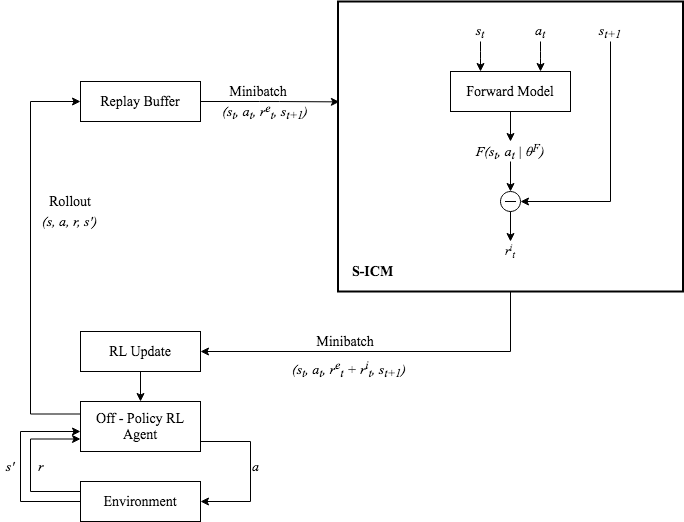
\includegraphics[scale=0.60]{review-0-architecture.png}
  \caption{Proposed System Architecture}
  \label{fig:proposed-system}
\end{figure}

The proposed system is a Curiosity-Driven Off-Policy agent which includes a modified version
of the ICM \textit{(Intrinsic Curiosity Module)} called the Simplified-ICM \cite{cdl2} coupled with a 
DQN based off-policy learner. The system is aimed at creating a sample-efficient method to train an agent to
navigate complex environments.

The environment to conduct the experiment in is 2D SuperMarioBros environment which 
has a continuous, non-repetitve state space in the form of pixel data with an 
extremely sparse reward system. The objective in this environment is to navigate to the 
end of the level while avoiding all obstacles. The complexity of this environment is attributed
to the fact that in a single level, a state will never occur more than once due to the
uni-directional nature of the level. This environment will be used as a baseline for comparison
with a much more complex 3D environment called MineRL with hierarchial tasks where the 
goal is to craft specific resources by gathering raw materials from the environment. The choice of the agent, 
DDDQN \textit{(Dueling Double Deep Q-Network)} \cite{duel}\cite{double} or DQfD \textit{(Deep Q-Learning from Demonstrations)} 
depends on the environment.

The agent initially observes the state $s$ of the environment and performs an action $a$ 
for which the environment returns a new state $s'$ and an extrinsic reward $r^e$. This experiences
tuple consisting of a state, action, reward and next state  $(s, a, r^e, s')$ is stored in a 
replay buffer which is a store for experience tuples. Independantly, the buffer is sampled 
by the S-ICM and it generates an intrinsic reward signal $r^i$ which is combined with 
the extrinsic reward and given to the agent to perform the TD \textit{(temporal difference)} update.
Based on this newly constructed reward signal, the TD update is performed. With these newly calculated
estimates, the agent will start to explore previously unseen states and find better 
solutions to the environment.

\section{Module Split-Up}

\subsection{Off-Policy Agent}
An Off-Policy agent was chosen for the project for two reasons. The relatively sample-efficient
nature of such algorithms due to the use of a Replay Buffer and due to the availability of 
human-demonstrations for the second environment which requires the aforementioned Replay Buffer.
The algorithm to be used will be a slight modification of the DQN called the DDDQN which has a 
better performance overall. The second environment will use a DQfD which doesn't have to interact with environment
as much as the batches of data are already present. The Q-Network in the agents will take in input in the 
form of stacked grayscale pixel-data (e.g. frames from 4 consecutive time steps stacked to form a 4 channel image) 
to preserve the characteristics of the change in the environment over time. The network produces two outputs. A single
value depicting the overall value of the state $V(s)$ and a tensor of action advantage values for every
action possible in the state $A^\pi(s,a) \forall a \in A$. The loss function used will be Huber Loss 
(SmoothL1Loss) as it is less sensitive to outliers in data than the squared error loss. This output 
is indirectly used by an $\epsilon$-greedy policy
to explore or exploit its current knowledge of the environment where the $\epsilon$ value
is reduced from 1.00 (completely random action) to 0.01 (99\% deterministic action) over 1,000,000
interactions with the environment.

\subsection{Simplified Intrinsic Curiosity Module}
This module is to be used in the pipeline in between the Replay Buffer and the agent to generate
a modified intrinsic reward signal as oppopsed to directly sending the batch of data from the Replay Buffer
to the agent for the TD update. The rewards stored in the Replay Buffer are from the environment and are sparse
and so the S-ICM generates a modified reward using which the TD update is performed by the agent.
This module is also used to make up for the drawback of DQN based agents which is their inability to generalize
to unseen states as evidence suggests that this module improves the ability of an agent to generalize.
The S-ICM consists of a neural network that takes in a state $s_t$ and an action $a_t$ and predicts the next state $s'_{t+1})$
which is compared with the actual next state $s_{t+1}$. The loss function used for this network is a 
mean squared error loss. The maginitude of the loss here shows its level
of knowledge about the dynamics of the environment. The higher the loss, the higher the intrinsic reward
which incentivizes a sense of "curiosity" in the agent to revisit the visited state and explore further.

\subsection{Replay Buffer}
The Replay Buffer is a collection of states $s$, actions $a$, extrinsic rewards $r^e$ and 
next states $s'$ which constitutes an experience tuple. The Buffer is uniformly sampled to 
create a batch of uncorellated experience tuples in a random order. There are multiple advantages
to doing this. First, each step of experience is potentially used in many weight 
updates, which allows for greater data efficiency. Second, learning directly from
consecutive samples is inefficient, owing to the strong correlations between the 
samples; randomizing the samples breaks these correlations and therefore reduces 
the variance of the updates. Third, when learning on-policy the current parameters 
determine the next data sample that the parameters are trained on. For example, if the
maximizing action is to move left then the training samples will be dominated by
samples from the left-hand side; if the maximizing action then switches to the 
right then the training distribution will also switch. 
It is easy to see how unwanted feedback loops may arise and the parameters could
get stuck in a poor local minimum, or even diverge catastrophically. The use of a Replay
Buffer avoids such scenarios.

\begin{thebibliography}{99}
\bibliographystyle{plain}

  \bibitem[1]{dqn}Mnih, V., Kavukcuoglu, K., Silver, D. et al. 
  {\em Human-level control through deep reinforcement learning.} 
   Nature 518, 529–533 (2015).

  \bibitem[2]{dqdf}Hester, T., Vecerik, M., Pietquin, 0., et al. 
  {\em Deep Q-learning from Demonstrations.}
  ArXiv (2017).

  \bibitem[3]{per}Schaul, T., Quan, J., Antonoglou, I., and Silver, D.
  {\em Prioritized Experience Replay.}
  ArXiv (2015).

  \bibitem[4]{ddpg}Lillicrap, T., Hunt, J., Pritzel, A. et al.
  {\em Continuous control with deep reinforcement learning.}
  ArXiv (2015).

  \bibitem[5]{td3}Fujimoto, S., Hoof, H., Meger, D.
  {\em Addressing Function Approximation Error in Actor-Critic Methods.}
  ArXiv (2018).

  \bibitem[6]{cdl} Pathak, D., Agrawal, P., Efros, A., Darrell, T.
  {\em Curiosity-Driven Exploration by Self-Supervised Prediction.}
  IEEE Conference on Computer Vision and Pattern Recognition Workshops (CVPRW) (2017).

  \bibitem[7]{her} Andrychowicz, M., Wolski, F., Ray, A.,
  {\em Hindsight Experience Replay.}
  Advances in Neural Information Processing Systems 30 (NIPS) (2017).

  \bibitem[8]{cdl2} B. Li, T. Lu, J. Li, N. Lu, Y. Cai and S. Wang, 
  {\em Curiosity-Driven Exploration for Off-Policy Reinforcement Learning Methods.}
  IEEE International Conference on Robotics and Biomimetics (ROBIO) (2019)

  \bibitem[9]{duel} Hasselt, H., Guez, A. and Silver, D., 
  {\em Dueling Network Architectures for Deep Reinforcement Learning.}
  ArXiv (2015).

  \bibitem[10]{double} Wang, Z., Freitas, N. and Lanctot, M. 
  {\em Deep Reinforcement Learning with Double Q-learning.}
  ArXiv (2015).

\end{thebibliography}
	
\end{document}
